\documentclass[conference]{IEEEtran}
% CVMI 2027 (IIITDM Kancheepuram), IEEE conference format. Check the CFP for page limit and
% whether review is double-blind (if so, replace the author block and anonymise the repo link).
\usepackage{cite}
\usepackage{amsmath,amssymb}
\usepackage{graphicx}
\usepackage{booktabs}
\usepackage{multirow}
\usepackage{xcolor}
\usepackage{pgfplots}
\pgfplotsset{compat=1.17}
\usetikzlibrary{positioning,arrows.meta,fit,calc}
\usepackage[hidelinks]{hyperref}

\newcommand{\dauc}{$\Delta$AUC}

\begin{document}

\title{Present, Attended, but Not Useful: A Pre-Registered Re-Examination of Neighbour Interaction Modelling for Pedestrian Crossing Prediction}

\author{\IEEEauthorblockN{Vikash Paigamber}
\IEEEauthorblockA{Department of Computer Science \& Engineering\\
Maulana Azad National Institute of Technology, Bhopal, India\\
% TODO: supervisor / co-authors, e-mail
}}

\maketitle

\begin{abstract}
Many pedestrian crossing-intention models add a module that reasons about surrounding road users, and report gains from it. We test whether such gains hold under a pre-registered protocol. On the PIE and JAAD\textsubscript{beh} time-to-event benchmarks (16 observed frames, 1--2\,s before the event), we compare a trajectory model with and without a neighbour-interaction transformer that is otherwise identical, using three seeds, a single locked test run per dataset and confidence intervals obtained by resampling pedestrian tracks. Neighbours are present in most test windows (86\% on PIE, 83\% on JAAD). Adding the interaction branch did not improve ROC-AUC on either dataset (PIE: $+0.002$, 95\% CI $[-0.008, +0.014]$; JAAD: $-0.040$, $[-0.097, +0.016]$); on PIE, gains as large as the pre-registered minimum of 0.015 lie outside the interval. Mechanism tests show that on PIE the model's attention does identify the neighbour its prediction depends on most (removal effect 2.5$\times$ that of a matched control, Holm-adjusted $p<10^{-4}$), but its response to neighbour motion follows motion magnitude rather than approach direction and is matched by a direction-scrambled placebo. Simple baselines explain why: a logistic regression on two apparent-speed features reaches 0.904 AUC on PIE and matches the deep model on JAAD (0.719 vs.\ 0.718). On these benchmarks, crossing prediction is dominated by the pedestrian's apparent motion, which leaves little room for interaction cues to add information.
\end{abstract}

\begin{IEEEkeywords}
pedestrian crossing intention, interaction modelling, pre-registration, shortcut learning, autonomous driving
\end{IEEEkeywords}

%=====================================================================
\section{Introduction}
Predicting whether a pedestrian will cross in front of a vehicle is a core perception task for automated driving. Since the release of JAAD~\cite{rasouli2017jaad} and PIE~\cite{rasouli2019pie}, models have grown from box-trajectory recurrent networks~\cite{rasouli2019sfgru} to multi-modal transformers~\cite{kotseruba2021benchmark}, and a common component is an explicit model of the surrounding road users, usually a graph or attention module over neighbouring pedestrians and vehicles~\cite{liu2020strr,yau2021graphsim,zhai2022social}, motivated by the view that crossing is negotiated with other road users~\cite{rasouli2020survey}. Such modules are typically justified by ablations in which removing them lowers a benchmark score. These ablations rarely report variation across seeds or confidence intervals, so it is often unclear how much of a reported gain would survive a repeated, controlled comparison~\cite{bouthillier2021variance,dodge2019showyourwork,henderson2018matters}.

For trajectory forecasting, where social interaction modelling is standard~\cite{alahi2016sociallstm,gupta2018socialgan,salzmann2020trajectron,kothari2022trajnet}, Makansi et al.~\cite{makansi2022walkalone} showed with Shapley-value attribution that state-of-the-art models use almost only the target's own past trajectory, and a constant-velocity model is a strong competitor~\cite{schoeller2020cvm}. Whether the same holds for crossing-intention \emph{classification}, where interaction modules are routinely reported to help, has not been tested under a controlled protocol to our knowledge.

We ask a narrower question: \emph{does modelling neighbours improve crossing prediction on the standard time-to-event benchmarks, and if not, why not?} We fix a protocol before evaluating the test split, compare two models that differ only in the neighbour branch, and test four pre-registered hypotheses on PIE and JAAD\textsubscript{beh}:
\begin{itemize}
  \item \textbf{H1}: neighbours are available in a minority of windows;
  \item \textbf{H2}: the interaction branch improves AUC; the locked primary test requires the 95\% CI of the overall \dauc{} to exclude zero and \dauc{} $\ge 0.015$, and the stratified form requires a gain where neighbours are present ($K\ge1$) but not where they are absent ($K=0$);
  \item \textbf{H3}: removing the neighbour that receives the highest attention changes the prediction more than removing a matched control neighbour;
  \item \textbf{H4}: speeding up approaching neighbours lowers the predicted crossing probability, more consistently than a placebo perturbation.
\end{itemize}

\noindent Our contributions are:
\begin{enumerate}
  \item A pre-registered, track-level test of neighbour-interaction utility on two benchmarks, which finds no gain and, on PIE, excludes gains of 0.015 AUC or more (Sec.~\ref{sec:h2}).
  \item Mechanism tests showing that the interaction model attends faithfully to specific neighbours (H3) but responds to their motion magnitude rather than direction (H4) (Sec.~\ref{sec:mech}).
  \item Simple-feature baselines that quantify the dominant cue: two apparent-speed numbers reach 0.904 AUC on PIE and match the deep model on JAAD (Sec.~\ref{sec:base}).
  \item Evidence that small validation splits can produce convincing but false gains: on JAAD the interaction model gained $+0.082$ AUC on validation and lost $0.040$ on test (Sec.~\ref{sec:rev}).
\end{enumerate}

%=====================================================================
\section{Related Work}
\textbf{Crossing intention benchmarks.} JAAD~\cite{rasouli2017jaad} and PIE~\cite{rasouli2019pie} provide per-frame pedestrian boxes and crossing annotations from dash-camera video. Kotseruba et al.~\cite{kotseruba2021benchmark} standardised the time-to-event (TTE) protocol used here, with 16 observed frames ending 1--2\,s before the crossing event, and found that performance varies strongly with ego-vehicle speed, partly because ego-motion changes how pedestrians appear to move in the image.

\textbf{Interaction modelling.} Graph-based and social-context models reason over pedestrians and surrounding objects to predict intent~\cite{liu2020strr,yau2021graphsim,zhai2022social}. Their benefit is typically supported by ablations on a single run. We test the same idea, a neighbour-attention branch, with matched models, several seeds, interval estimates and controls.

\textbf{Simple cues and shortcuts.} Achaji et al.~\cite{achaji2022bbox} showed that transformers using bounding boxes alone are competitive on PIE and JAAD, and a permutation feature-importance study found bounding boxes and ego-vehicle speed to be the dominant inputs, with signs of speed-related bias~\cite{featureimportance2024}. More generally, models often exploit the easiest available signal~\cite{geirhos2020shortcut}. In trajectory forecasting, interaction features contribute little to state-of-the-art models~\cite{makansi2022walkalone}, constant-velocity extrapolation is hard to beat~\cite{schoeller2020cvm}, separating ego-motion from pedestrian motion lets simple models compete with complex ones~\cite{neumann2021egomotion}, and counterfactual interventions have been used to reduce a predictor's reliance on environment cues~\cite{chen2021counterfactual}. Our study asks the corresponding question for crossing-intention classification on PIE and JAAD, replaces post-hoc attribution with pre-registered matched interventions, and links the interaction branch's behaviour to the apparent-motion cue.

\textbf{Attention as explanation and pre-registration.} Whether attention weights or saliency maps reflect what a model uses is debated~\cite{jain2019attention,wiegreffe2019attention,adebayo2018sanity}; H3 tests this with matched interventions. Pre-registration, i.e.\ fixing hypotheses and analysis before seeing outcome data, guards against analytic flexibility~\cite{nosek2018prereg}, a recurring concern in machine-learning evaluation~\cite{lipton2019troubling,kapoor2023leakage}.

%=====================================================================
\section{Protocol, Data and Models}

\subsection{Pre-registration}
Hypotheses H1--H4, their decision rules and Holm correction~\cite{holm1979} were written on 28~Sep~2026, before the models in this paper were trained. The primary H2 analysis (overall \dauc{} of seed ensembles, minimum meaningful effect 0.015, 2{,}000 track-bootstrap resamples) was then locked in version control (commit \texttt{36bd0c5}) before the PIE test split was evaluated, and the test evaluation was run exactly once. JAAD was locked separately (commit \texttt{de82a59}) after its validation run and before its test run; the PIE result was known at that point. H1, H3 and H4 were evaluated afterwards following the 28~Sep specification, and are therefore exploratory with respect to the lock. Earlier versions of this pipeline, which used a different labelling, a wrong time step and placeholder visual inputs, also touched PIE Set~03; all of those results were discarded. Deviations from the 28~Sep document are listed in Sec.~\ref{sec:lim}. Code and the locked protocol documents are available at \url{https://github.com/vikaxxh/explainable-multimodal-HAR}.

\subsection{Data}
We follow the TTE windowing of~\cite{kotseruba2021benchmark}, with one difference noted below. A window holds 16 observed frames (30\,fps) whose last frame lies 30--60 frames before the event: the first frame annotated \emph{crossing} for crossing pedestrians, and the last annotated frame otherwise. This event definition for non-crossing pedestrians is our own choice and may differ from the reference implementation of~\cite{kotseruba2021benchmark}; absolute AUCs are therefore not directly comparable with published results. Windows are sampled with 60\% overlap; pedestrians annotated only as \emph{crossing-irrelevant} are excluded. PIE uses the official split (train Sets 01/02/04, validation 05/06, test 03); JAAD\textsubscript{beh} uses the official video-disjoint split. Inputs are box-centre kinematics $[x, y, v_x, v_y, \theta]$ in image coordinates normalised by each clip's resolution. Up to four neighbours are kept: agents annotated in all 16 frames whose mean distance to the pedestrian is at most 0.20 (PIE: pedestrians and vehicles; JAAD: pedestrians only, since JAAD has no vehicle boxes). $K$ denotes the number of neighbours at the last observed frame. The PIE test split contains 3{,}886 windows from 675 tracks (26\% crossing windows); the JAAD test split has 829 windows from 154 tracks (49\%). Validation splits are 1{,}320 windows / 227 tracks (PIE) and 149 / 28 (JAAD). Automated checks confirmed that no track appears in more than one split and that every time-to-event lies within 30--60 frames.

\subsection{Models}
\begin{figure}[t]
\centering
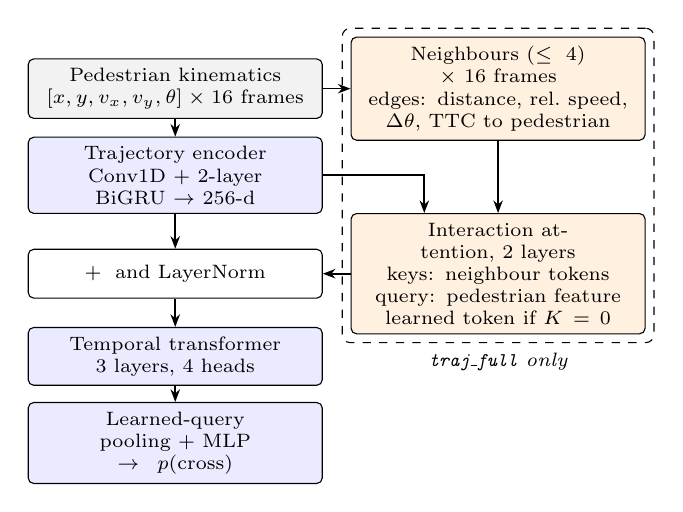
\begin{tikzpicture}[font=\scriptsize,
  blk/.style={draw, rounded corners=2pt, align=center, text width=3.5cm, minimum height=0.62cm, fill=#1},
  blk/.default=white, arr/.style={-{Stealth[length=1.6mm]}, semithick}]
% shared path (both models)
\node[blk=gray!10] (ped) at (0,0) {Pedestrian kinematics\\$[x,y,v_x,v_y,\theta]\times16$ frames};
\node[blk=blue!8] (enc) at (0,-1.1) {Trajectory encoder\\Conv1D + 2-layer BiGRU $\rightarrow$ 256-d};
\node[blk=white] (add) at (0,-2.35) {$+$ \;and LayerNorm};
\node[blk=blue!8] (tmp) at (0,-3.4) {Temporal transformer\\3 layers, 4 heads};
\node[blk=blue!8] (head) at (0,-4.5) {Learned-query pooling + MLP\\$\rightarrow p(\text{cross})$};
% interaction branch (traj_full only)
\node[blk=orange!12] (nb) at (4.1,0) {Neighbours ($\le4$) $\times$ 16 frames\\edges: distance, rel.\ speed,\\$\Delta\theta$, TTC to pedestrian};
\node[blk=orange!12] (att) at (4.1,-2.35) {Interaction attention, 2 layers\\keys: neighbour tokens\\query: pedestrian feature\\learned token if $K=0$};
\node[draw, dashed, rounded corners=3pt, inner sep=3pt, fit=(nb)(att),
      label={[font=\scriptsize\itshape]below:\texttt{traj\_full} only}] (box) {};
% arrows
\draw[arr] (ped) -- (enc);
\draw[arr] (enc) -- (add);
\draw[arr] (add) -- (tmp);
\draw[arr] (tmp) -- (head);
\draw[arr] (ped.east) -- (nb.west);
\draw[arr] (nb) -- (att);
\draw[arr] (enc.east) -| ($(att.north west)!0.25!(att.north east)$);
\draw[arr] (att.west) -- (add.east);
\end{tikzpicture}
\caption{The two models. Both share the trajectory encoder, temporal transformer and crossing head. \texttt{traj\_full} adds the interaction branch (dashed): at each frame the pedestrian feature attends over its neighbours, and the result is added to the pedestrian feature and layer-normalised. \texttt{traj\_isolated} omits the branch and the addition.}
\label{fig:arch}
\end{figure}

Both models (Fig.~\ref{fig:arch}) share a trajectory encoder (1-D temporal convolution followed by a 2-layer bidirectional GRU~\cite{cho2014gru} with 128 hidden units in total, projected to 256 dimensions), a 3-layer temporal transformer~\cite{vaswani2017attention} (4 heads) and a crossing head that pools over time with a learned query. \texttt{traj\_full} adds a 2-layer interaction transformer in which the pedestrian attends to its neighbours, using per-pair edge features (distance, relative velocity, heading difference, time-to-collision); neighbour tokens are embedded from the neighbours' own kinematics, a learned token replaces the neighbour set when $K=0$, and the result is added residually to the pedestrian features followed by layer normalisation. \texttt{traj\_isolated} omits this branch and is otherwise identical. Both are trained with focal loss~\cite{lin2017focal} ($\alpha=0.75$, $\gamma=2$, label smoothing 0.05), AdamW~\cite{loshchilov2019adamw} (learning rate $10^{-4}$, weight decay 0.01, cosine annealing to $10^{-6}$ over at most 60 epochs, no warm-up), batch size 32, dropout 0.3, horizontal-flip augmentation applied jointly to the pedestrian and its neighbours and early stopping on validation AUC (patience 10), with seeds 42, 100 and 2024, on CPU. The hyper-parameters were identical for both datasets and not tuned on any test split.

\subsection{Statistics}
Each comparison uses the seed-ensemble (mean) probability of each model. Confidence intervals for \dauc{} come from a paired bootstrap that resamples pedestrian tracks (2{,}000 resamples for the locked H2 analysis, 1{,}000 for H1--H4), since windows from one track are correlated~\cite{efron1993bootstrap}. Strata with fewer than 25 tracks are treated as descriptive only. Two neighbour controls are applied to \texttt{traj\_full}: \emph{removed} (all neighbours masked) and \emph{shuffled} (neighbour sets taken from windows of other tracks).

%=====================================================================
\section{Results}

\subsection{H1: Neighbours are common}
Neighbours are present in most windows: $K\ge1$ in 85.6\% of PIE test windows (95\% CI [83.3, 88.0]) and 83.2\% of JAAD test windows ([77.1, 88.5]); 67.6\% and 63.8\% have two or more. H1's prediction of sparsity is therefore refuted. A null result for H2 cannot be attributed to a lack of neighbours.

\subsection{H2: No gain from the interaction branch}\label{sec:h2}

\begin{table}[t]
\centering
\caption{Test-set performance (per-seed mean $\pm$ s.d., 3 seeds; nbrs.: neighbours of the interaction model).}
\label{tab:main}
\footnotesize
\setlength{\tabcolsep}{3pt}
\begin{tabular}{@{}llccc@{}}
\toprule
 & Model & AUC & PR-AUC & Brier \\
\midrule
\multirow{4}{*}{PIE} & Isolated & $0.947\pm.000$ & $0.823\pm.008$ & $0.131\pm.004$ \\
 & Interaction & $0.948\pm.003$ & $0.842\pm.016$ & $0.108\pm.004$ \\
 & \quad nbrs.\ removed & $0.947\pm.001$ & $0.845\pm.003$ & $0.118\pm.004$ \\
 & \quad nbrs.\ shuffled & $0.907\pm.007$ & $0.724\pm.025$ & $0.134\pm.004$ \\
\midrule
\multirow{4}{*}{JAAD} & Isolated & $0.718\pm.016$ & $0.693\pm.023$ & $0.236\pm.005$ \\
 & Interaction & $0.680\pm.028$ & $0.663\pm.022$ & $0.276\pm.016$ \\
 & \quad nbrs.\ removed & $0.712\pm.021$ & $0.687\pm.022$ & $0.237\pm.012$ \\
 & \quad nbrs.\ shuffled & $0.693\pm.024$ & $0.678\pm.018$ & $0.267\pm.021$ \\
\bottomrule
\end{tabular}
\end{table}

\begin{table}[t]
\centering
\caption{\dauc{} (interaction $-$ comparison), seed ensembles, 95\% track-bootstrap CI.}
\label{tab:delta}
\footnotesize
\setlength{\tabcolsep}{3pt}
\begin{tabular}{@{}lcc@{}}
\toprule
Comparison & PIE (675 tracks) & JAAD (154 tracks) \\
\midrule
vs.\ isolated, all & $+0.002$ [$-0.008$, $+0.014$] & $-0.040$ [$-0.097$, $+0.016$] \\
vs.\ isolated, $K=0$ & $+0.001$ [$-0.009$, $+0.011$] & $-0.057$ [$-0.141$, $+0.021$] \\
vs.\ isolated, $K\ge1$ & $+0.003$ [$-0.008$, $+0.017$] & $-0.038$ [$-0.100$, $+0.024$] \\
vs.\ removed, all & $+0.001$ [$-0.009$, $+0.014$] & $-0.031$ [$-0.096$, $+0.029$] \\
vs.\ shuffled, all & $+0.041$ [$+0.029$, $+0.053$] & $-0.016$ [$-0.072$, $+0.038$] \\
\bottomrule
\end{tabular}
\end{table}

\begin{figure}[t]
\centering
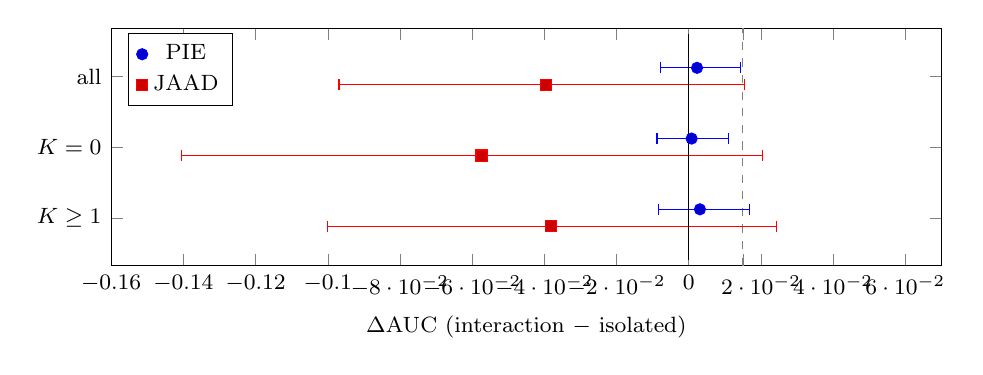
\begin{tikzpicture}
\begin{axis}[
  width=\columnwidth, height=4.6cm, xmin=-0.16, xmax=0.07,
  xlabel={\dauc{} (interaction $-$ isolated)}, ytick={1,2,3}, yticklabels={$K\ge1$,$K=0$,all},
  y dir=normal, enlarge y limits=0.25, legend style={at={(0.02,0.98)},anchor=north west,font=\footnotesize},
  tick label style={font=\footnotesize}, label style={font=\footnotesize},
  extra x ticks={0.015}, extra x tick labels={}, extra x tick style={grid=major, grid style={dashed,gray}},
  xmajorgrids=false]
\addplot+[only marks, mark=*, color=blue, error bars/.cd, x dir=both, x explicit]
  coordinates {(0.0031,1.12) -= (0.0114,0) += (0.0137,0)
               (0.0008,2.12) -= (0.0096,0) += (0.0103,0)
               (0.0023,3.12) -= (0.0101,0) += (0.0120,0)};
\addplot+[only marks, mark=square*, color=red, error bars/.cd, x dir=both, x explicit]
  coordinates {(-0.0382,0.88) -= (0.0620,0) += (0.0624,0)
               (-0.0574,1.88) -= (0.0831,0) += (0.0779,0)
               (-0.0395,2.88) -= (0.0574,0) += (0.0550,0)};
\draw[black] (axis cs:0,0.4) -- (axis cs:0,3.6);
\legend{PIE, JAAD}
\end{axis}
\end{tikzpicture}
\caption{H2: \dauc{} with 95\% track-bootstrap CIs. The dashed line marks the pre-registered minimum meaningful effect (0.015).}
\label{fig:h2}
\end{figure}

On PIE, \texttt{traj\_full} and \texttt{traj\_isolated} reach nearly identical AUC (Table~\ref{tab:main}). The seed-ensemble \dauc{} is $+0.0023$ (95\% CI $[-0.0078, +0.0143]$, $p=0.69$; Table~\ref{tab:delta}, Fig.~\ref{fig:h2}), so the locked H2 test is not supported. The upper end of the interval lies below the pre-registered minimum meaningful effect of 0.015: gains of that size are not compatible with the data at the 95\% level. This is a descriptive reading of the interval; the locked rule was a superiority test, not a formal equivalence test~\cite{lakens2017equivalence}. The difference is near zero both for $K=0$ and $K\ge1$, so the stratified form of H2 (gain at $K\ge1$ only) is not supported either. On JAAD the point estimate is negative ($-0.040$, $[-0.097, +0.016]$). Neither form of H2 is supported on either dataset, with or without Holm correction.

The interaction model is better calibrated on PIE (Brier 0.108 vs.\ 0.131) and has a slightly higher PR-AUC, but its F1 at a fixed 0.5 threshold is lower (\,$\Delta$F1 $-0.022$, CI $[-0.044, -0.001]$; JAAD $-0.043$, $[-0.066, -0.021]$). Because AUC, which does not depend on a threshold, is unchanged, we read this as a shift in the predicted probabilities relative to the threshold rather than worse discrimination.

The controls show that the PIE model does read its neighbour inputs: replacing neighbours with those of other tracks lowers AUC by 0.041 ($[0.029, 0.053]$), while removing them changes nothing ($+0.001$). Correct neighbours therefore add essentially nothing beyond the trajectory, but wrong ones hurt. Shuffled neighbours keep their own image coordinates and can lie farther from the pedestrian than any training neighbour, so part of this drop may reflect unusual inputs rather than wrong interactions.

\subsection{H3 and H4: Faithful attention, non-directional response}\label{sec:mech}

\begin{table}[t]
\centering
\caption{Mechanism tests on the test splits (seed ensembles).}
\label{tab:mech}
\footnotesize
\setlength{\tabcolsep}{4pt}
\begin{tabular}{@{}lcc@{}}
\toprule
 & PIE & JAAD \\
\midrule
\multicolumn{3}{@{}l}{\emph{H3: remove top-attended vs.\ matched neighbour}} \\
Matched windows / tracks & 709 / 210 & 168 / 51 \\
Mean $|\Delta p|$ target / control & 0.025 / 0.010 & 0.032 / 0.025 \\
Median $\delta$ & $+0.0034$ & $+0.0040$ \\
\quad 95\% CI & [$+0.0018$, $+0.0054$] & [$+0.0008$, $+0.0082$] \\
Target is most influential & 52\% & 32\% \\
Wilcoxon~\cite{wilcoxon1945} $p$, track means & $2\times10^{-16}$ & 0.11 \\
\midrule
\multicolumn{3}{@{}l}{\emph{H4: rescale approaching neighbours' motion}} \\
Approaching units & 2{,}250 & 575 \\
Median $\rho$, real / placebo & $-0.20$ / $-1.00$ & $+0.49$ / $+0.83$ \\
Expected sign, real / placebo & 44.6\% / 60.0\% & 33.6\% / 29.2\% \\
McNemar~\cite{mcnemar1947} $p$, one-sided & 1.00 & 0.061 \\
Mahalanobis, orig.\ / $\alpha{=}2$ & 2.00 / 2.87 & 1.96 / 2.77 \\
\midrule
Holm $p$: H2 / H3 / H4 & 1.00 / $<10^{-4}$ / 1.00 & 0.47 / 0.34 / 0.24 \\
\bottomrule
\end{tabular}
\end{table}

\textbf{H3.} For windows with at least two neighbours, we remove the neighbour with the highest attention weight (last interaction layer, averaged over heads, frames and seeds) and, separately, a control neighbour matched on distance ($\pm$15\% or $\pm$0.05), speed ($\pm$20\%) and heading ($\pm30^\circ$), and compare $\delta = |\Delta p_{\text{target}}| - |\Delta p_{\text{control}}|$. On PIE, removing the attended neighbour moves the prediction 2.5 times as much as removing the control (Table~\ref{tab:mech}); the median $\delta$ is positive with a CI excluding zero, and the Wilcoxon signed-rank test~\cite{wilcoxon1945} on track means is significant after Holm correction. H3 is supported on PIE: the attention identifies the neighbour the prediction depends on most, about half of the time the single most influential one. On JAAD the effect has the same sign but is not significant ($p=0.11$, 51 tracks). The absolute effects are small; removing the most influential neighbour changes $p$ by 0.034 on average on PIE. Only 27\% of eligible PIE windows had a matched control, so H3 describes a subset of scenes.

\textbf{H4.} For each window--neighbour pair we rescale the neighbour's trajectory around its last observed position, $\mathbf{p}'(t)=\mathbf{p}(T)-\alpha(\mathbf{p}(T)-\mathbf{p}(t))$, $\mathbf{v}'=\alpha\mathbf{v}$, for $\alpha\in\{0.5,\dots,2\}$, and compute Spearman $\rho$ between $\alpha$ and $p$. As a placebo, the same rescaling is applied after rotating the neighbour's displacement and velocity by a random angle, which keeps the motion magnitude but scrambles its direction relative to the pedestrian. On PIE, faster approaching neighbours lower $p$ slightly (median $\rho=-0.20$), but the placebo does so more consistently ($-1.00$), and receding neighbours show the same trend ($-0.43$). H4 is not supported: the model responds to how much neighbours move, not to whether they approach. On JAAD the response is positive for both real and placebo perturbations. The perturbed inputs remain close to the training distribution (Mahalanobis distance 2.87 at $\alpha=2$ vs.\ 2.00 unperturbed; $<0.1$\% of values outside the training range on PIE), so these responses are not caused by out-of-distribution inputs.

\subsection{What the models rely on}\label{sec:base}

\begin{table}[t]
\centering
\caption{Simple-feature baselines (test AUC, 95\% track-bootstrap CI; exploratory). LR: logistic regression, GB: gradient boosting.}
\label{tab:base}
\footnotesize
\setlength{\tabcolsep}{3pt}
\begin{tabular}{@{}lcc@{}}
\toprule
Features & PIE & JAAD \\
\midrule
Box size (GB) & 0.617 [0.577, 0.655] & 0.533 [0.472, 0.595] \\
Position (LR) & 0.648 [0.600, 0.693] & 0.574 [0.483, 0.666] \\
Speed, 2 features (LR) & 0.904 [0.881, 0.926] & 0.719 [0.641, 0.787] \\
Motion, 9 features (LR) & 0.942 [0.925, 0.957] & 0.728 [0.647, 0.797] \\
Motion, 9 features (GB) & 0.943 [0.930, 0.955] & 0.743 [0.677, 0.805] \\
\midrule
Deep, isolated / interaction & 0.947 / 0.948 & 0.718 / 0.680 \\
\bottomrule
\end{tabular}
\end{table}

To find the signal the models exploit, we fit logistic regression and gradient boosting on hand-crafted summaries of the observed window (Table~\ref{tab:base}). Position and box size are weak. Two numbers, the mean and last-frame apparent speed, give 0.904 AUC on PIE and 0.719 on JAAD, the latter matching the deep isolated model. Nine motion summaries (box-height growth, mean and spread of velocity, displacement, mean and last-frame speed) bring a linear model within 0.005 AUC of the deep models on PIE. On PIE, crossing pedestrians move about five times less in the image than non-crossing ones over the observed window (median speed 0.014 vs.\ 0.072 normalised units per second). A likely contributor is ego-motion: non-crossing tracks end as the vehicle passes the pedestrian, so the pedestrian sweeps across the image, whereas before a crossing the vehicle is typically slowing or stopped~\cite{kotseruba2021benchmark}. The H4 result fits this reading: the interaction model treats neighbour motion magnitude, which ego-motion also inflates, as evidence against crossing. We stress that we did not test the ego-motion explanation directly (e.g.\ with PIE's vehicle speed data). These baselines were run after the lock and are exploratory; we did not test the deep--simple differences statistically.

\subsection{Validation can mislead on small splits}\label{sec:rev}
On JAAD's 28-track validation split, the interaction model appeared clearly better ($+0.082$ AUC, $[-0.054, +0.238]$) and appeared to depend on its neighbours (removing them cost 0.123). On the 154-track test split the sign reversed ($-0.040$), and the interaction model was also worse for pedestrians without neighbours ($K=0$: $-0.057$), which points to overfitting of the larger model on 161 training tracks rather than to misused neighbours. Selecting checkpoints and drawing conclusions from such a small validation split is unreliable, and single-run ablations on JAAD-sized data should be read with caution. PIE, with 227 validation tracks, was consistent between validation ($+0.007$) and test ($+0.002$).

%=====================================================================
\section{Discussion}
The results fit one picture. Neighbours are present (H1), and the PIE model uses specific ones, since shuffling hurts and the attention points at the influential neighbour (H3). But this sensitivity follows motion magnitude rather than interaction geometry (H4), and it adds no predictive value (H2). The most plausible reason is that the benchmark's signal is already carried by the pedestrian's own apparent motion, which the trajectory branch captures; additional agents mostly repeat the same ego-motion-related cue; the interaction branch embeds each neighbour's own image-plane motion, which ego-motion inflates in the same way. Two practical points follow. First, gains attributed to interaction modules on these benchmarks should be checked against matched ablations with interval estimates and against simple motion baselines. Second, attention maps of interaction modules can be faithful, in the sense of H3, and still fail to reflect behaviourally meaningful reasoning; faithfulness is not the same as plausibility.

\section{Limitations}\label{sec:lim}
Our models use trajectories only; visual context, pose and the ego-vehicle's own speed may let interaction cues help, and our conclusions are limited to kinematic interaction under the TTE protocol. We evaluate one interaction architecture, not published third-party models. JAAD is small, so its intervals are wide, and its neighbours are pedestrians only, which makes H4 a weak test there. H3 covers only windows with a matched control. Relative to the 28~Sep protocol we used three seeds instead of five, selected checkpoints by maximum validation AUC instead of minimum validation loss, and used 2{,}000 bootstrap resamples for the locked H2 analysis; the H4 placebo implements the protocol's ``scrambled position'' perturbation as a random rotation of the neighbour's motion. H1, H3, H4 and the baselines were evaluated after the CVMI lock. Coordinates are normalised image coordinates, not metric distances. Defining the non-crossing event as the last annotated frame ties non-crossing windows to the end of a track, which may strengthen the apparent-motion cue of Sec.~\ref{sec:base}; our absolute AUCs should not be compared directly with published PIE/JAAD numbers.

\section{Conclusion}
Under a pre-registered protocol, an interaction-aware trajectory model did not predict pedestrian crossing better than an otherwise identical isolated model on PIE or JAAD, although neighbours were common and, on PIE, the model attended to the neighbour that mattered most. Apparent pedestrian speed explains most of what the benchmarks reward. Evaluating interaction models on scenes where kinematics are uninformative, and with ego-motion compensated, is a natural next step.

\bibliographystyle{IEEEtran}
\bibliography{refs}

\end{document}
